\section{Backend}


\begin{frame}{Backend}
	\begin{itemize}
		\item[] Python Server mit Flask API
		\begin{itemize}
			\itemsep 4pt
			\item stellt Endpunkte zum Persistieren der Stammdaten
			\item stellt Endpunkte zur Live Administration einer Übung
			\item stellt Endpunkte zur Teilnahme an einer Übung
		\end{itemize}
	\end{itemize}
\end{frame}


\begin{frame}{Backend-Komponenten}
	\centering
	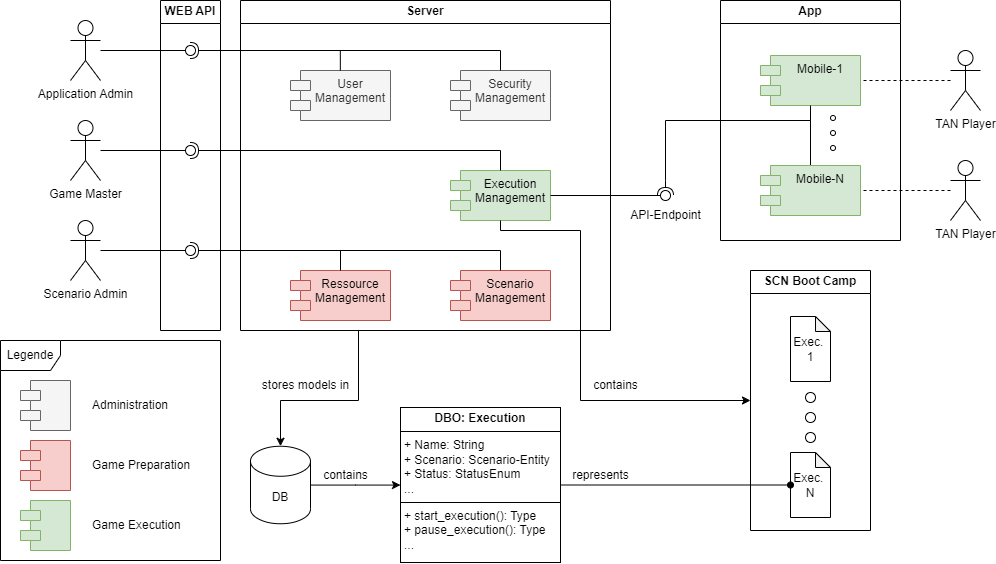
\includegraphics[width=0.7\textwidth]{images/server/component_diagram.png}
\end{frame}


\begin{frame}{Server: Datenhaltung}
	\begin{columns}
		\column{0.7\linewidth}
			\begin{itemize}
				\itemsep 12pt
				\item[] Trennung von Basis- und Spieldaten
				\begin{itemize}
					\itemsep 2pt
					\item[$\rightarrow$] In-memory Objekte für Spieldaten
					\item[$\rightarrow$] Datenbank für Template-Objekte   
				\end{itemize}
				\item[] Vorteile:
				\begin{itemize}
					\itemsep 2pt
					\item Unabhängigkeit von ORM
					\item Konstante schnelle Zugriffszeiten
					\item Kapselung
				\end{itemize}
				\item[] Nachteile:
				\begin{itemize}
					\itemsep 2pt
					\item Erhöhte Komplexität
					\item Synchronisation
				\end{itemize}
			\end{itemize}
		\column{0.3\linewidth}
			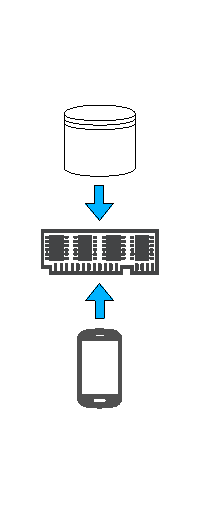
\includegraphics[height=\textheight]{images/server/datenhaltung.pdf}
	\end{columns} 
\end{frame}


\begin{frame}{Server: Laufzeitobjekte}
	\centering
	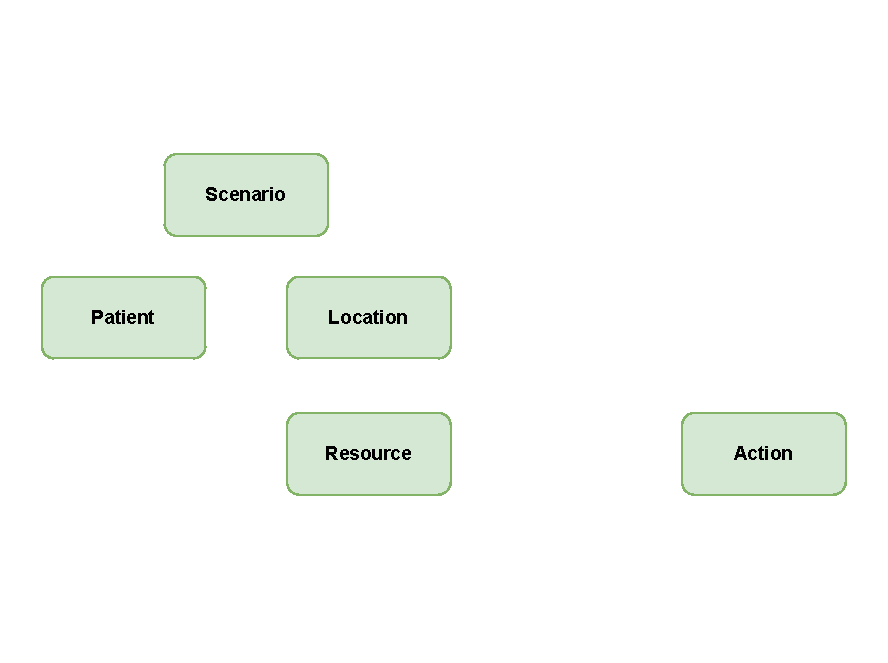
\includegraphics[height=.9\textheight]{images/server/laufzeit_objekte_1.pdf}
\end{frame}

\begin{frame}{Server: Laufzeitobjekte}
	\centering
	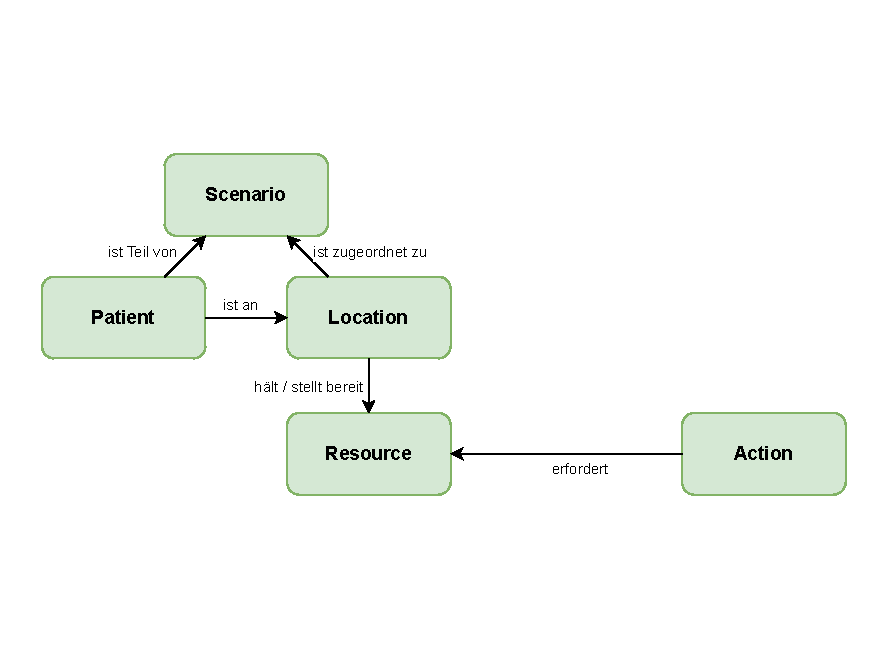
\includegraphics[height=.9\textheight]{images/server/laufzeit_objekte_2.pdf}
\end{frame}

\begin{frame}{Server: Laufzeitobjekte}
	\centering
	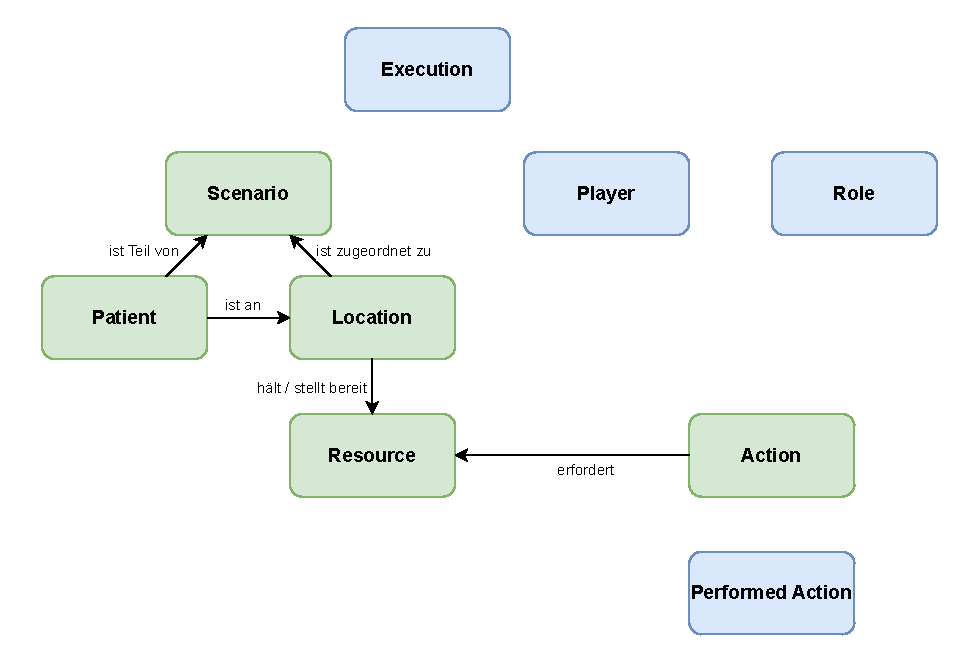
\includegraphics[height=.9\textheight]{images/server/laufzeit_objekte_3.pdf}
\end{frame}

\begin{frame}{Server: Laufzeitobjekte}
	\centering
	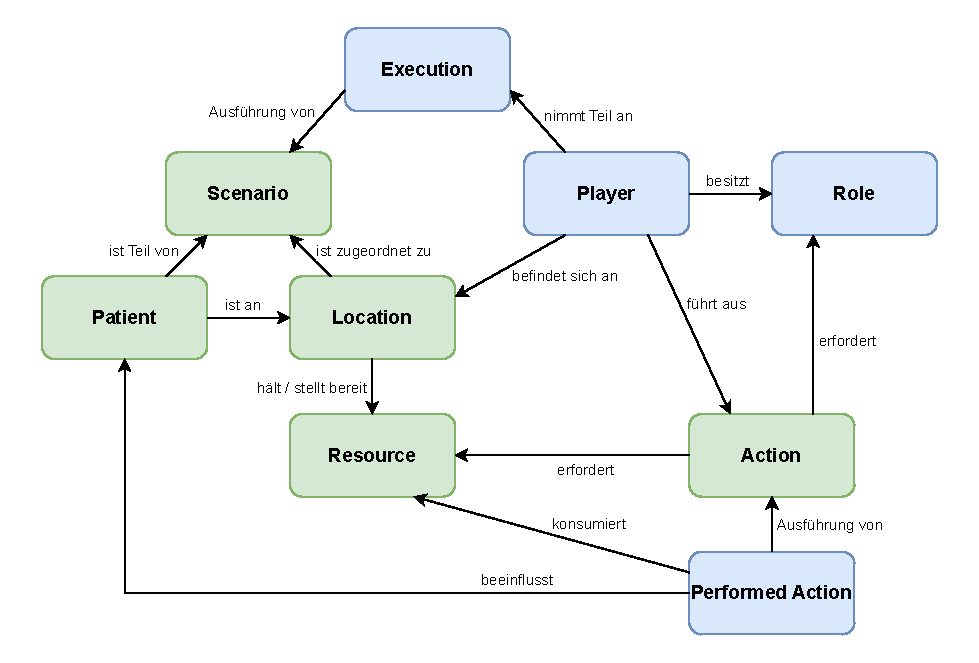
\includegraphics[height=.9\textheight]{images/server/laufzeit_objekte.pdf}
\end{frame}


\begin{frame}{Server: Datenbankobjekte}
	\centering
	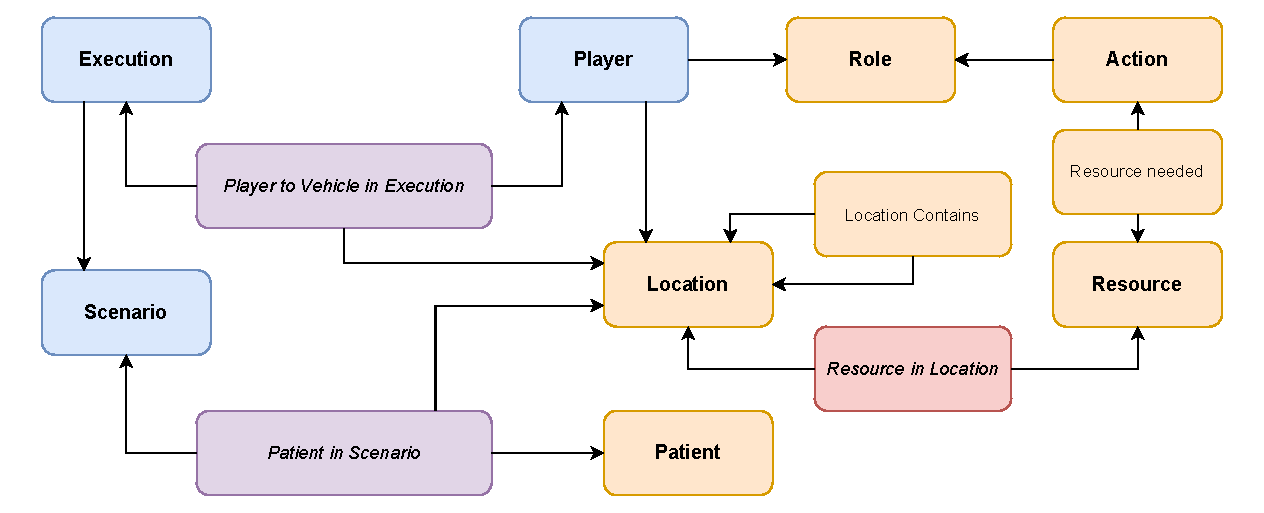
\includegraphics[width=\textwidth]{images/server/datenbank_objekte.pdf}
\end{frame}
